\section{Results}
\label{results}
In this section we present both the objective and the subjective results obtained. The outliers were taken out of the calculations.

\subsection{Objective Results}
\label{results_objective}
Table \ref{table:results_no_ext_f0_glott} shows the objective scores obtained for the synthetic speech of the GlottHMM-based system without using the external $F_{0}$ in the feature extraction.
%
The clean samples have been synthesized with the clean configuration while in all the noisy cases the noise reduction configuration was used. 

On the other hand, in Table \ref{table:results_ext_f0_glott} the results for all the noisy cases adapted using the external $F_{0}$ are presented.
%
In this case, there is no clean row, as the $F_{0}$ is calculated from the clean samples.
%
All the adaptations in this table were done with the noise reduction configuration.

As it can be seen, there are no significant differences between both approaches, what could lead us to think we can use either of them and obtain the same results.
%
However, when listening to the synthesized audio samples it becomes pretty clear that when not using an external $F_{0}$ there is a huge quality drop.
%
Therefore, not using an external $F_{0}$ is been rejected from this point on.

\begin{table}[!htb]
\begin{center}
\begin{tabular}{c c | c | c}
Noise & SNR & fwS & MCD\\
\midrule
\midrule
Clean & - & 9.0 & 1.8\\
\midrule
\multirow{3}{*}{Babble} & 20 & 10.6 & 3.0\\
 & 10 & 7.5 & 2.7\\
 & 5 & 6.3 & 2.6\\
\midrule
\multirow{2}{*}{Factory} & 10 & 6.8 & 3.0\\
 & 5 & 5.3 & 3.2\\
\midrule
Machine gun & 0 & 9.3 & 2.7\\
\midrule
\midrule
\multirow{2}{*}{Enhanced} & 20 & 10.8 & 3.0\\
\multirow{2}{*}{Babble} & 10 & 8.4 & 2.8\\
& 5 & 6.9 & 2.8\\
\midrule
Enhanced & 10 & 8.7 & 3.2\\
Factory & 5 & 7 & 3.3\\
\bottomrule
\end{tabular}
\caption{Objective scores for the adapted test data using the $F_{0}$ calculated for each case with the GlottHMM-based system}
\label{table:results_no_ext_f0_glott}
\end{center}
\end{table}

In Table \ref{table:comp_adapt_results} the comparison between the GlottHMM and STRAIGHT systems can be evaluated through the objective scores.
%
The above result in the clean row is obtained with the clean configuration of GlottHMM, while the one below is obtained using the noise reduction configuration.
%
The contradictory results in the case of the GlottHMM-based system still happening: when SNR shows an improvement the MCD shows a quality decrease.
%
Also, the GlottHMM-based system is found to suffer more degradation under severe noise conditions than the STRAIGHT one.
%
We can spot that the noise reduction system makes the MCD values to increase, as so as the SNR values, giving the contradictory results previously seen.

In all the objective scores, GlottHMM presents a significantly steeper drop in quality as the noise level increases.
%
This drop is clearly audible for SNR 5dB. 

\begin{table}[!htb]
\begin{center}
\begin{tabular}{c c | c | c}
Noise & SNR & fwS & MCD\\
\midrule
\midrule
\multirow{3}{*}{Babble} & 20 & 10.7 & 3.0\\
 & 10 & 7.6 & 2.7\\
 & 5 & 6.4 & 2.7\\
\midrule
\multirow{2}{*}{Factory} & 10 & 6.9 & 2.9\\
 & 5 & 5.5 & 3.2\\
\midrule
Machine gun & 0 & 9.4 & 2.7\\
\midrule
\midrule
\multirow{2}{*}{Enhanced} & 20 & 10.6 & 3.0\\
\multirow{2}{*}{Babble} & 10 & 8.4 & 2.8\\
& 5 & 6.8 & 2.7\\
\midrule
Enhanced & 10 & 8.7 & 3.2\\
Factory & 5 & 7.1 & 3.3\\
\bottomrule
\end{tabular}
\caption{Objective scores for the adapted test data using an external in the feature extraction $F_{0}$ calculated from the clean data with the GlottHMM-based system}
\label{table:results_ext_f0_glott}
\end{center}
\end{table}

\begin{table}[htb]
\begin{centering}
\begin{tabular}{c c|c c|c c}
	 & & \multicolumn{2}{c|}{Adapted} & \multicolumn{2}{c}{Adapted}\\
	 & & \multicolumn{2}{c|}{GlotHMM} & \multicolumn{2}{c}{STRAIGHT}\\
	 & & \multicolumn{2}{c|}{synthesized} & \multicolumn{2}{c}{synthesized}\\
	 & & \multicolumn{2}{c|}{test data} & \multicolumn{2}{c}{test data}\\
	Noise & SNR & fwS & MCD & fwS & MCD\\
	\midrule
	\midrule
	\multirow{2}{*}{Clean} & \multirow{2}{*}{-} & 9.0 & 1.8 & \multirow{2}{*}{7.5} & \multirow{2}{*}{2.1}\\
	 & & 10.6 & 2.9 & & \\	
	\midrule
	\multirow{3}{*}{Babble} & 20 & 10.7 & 3 & 8.0 & 2.0\\
	 & 10 & 7.6 & 2.7 & 7.5 & 2.1\\
	 & 5 & 6.4 & 2.7 & 7.3 & 2.2\\
	\midrule
	\midrule
	\multirow{2}{*}{Enhanced} & 20 & 10.6 & 3.0 & 8.0 & 2.0\\
	\multirow{2}{*}{Babble} & 10 & 8.4 & 2.8 & 7.5 & 2.1\\
	 & 5 & 6.8 & 2.7 & 7.3 & 2.2\\
	\bottomrule
\end{tabular}
\caption{Objective scores comparing GlottHMM and STRAIGHT}
\label{table:comp_adapt_results}
\end{centering}
\end{table}

\subsection{Subjective Results}
\label{results_subjective}
In the listening test two male voices were evaluated for different vocoders adaptation and different GlottHMM configurations by 32 native speakers using a web-based test.
%
The results for both speakers were similar enough to be grouped.

In the AB test two different comparison where made.
%
The first one asked the listeners about their preferences between different synthetic speech obtained with the GlottHMM-based system.
%
The cases faced were:

\begin{itemize}
	\item Adapted speech from clean data using the clean configuration against adapted speech from clean data using the noise reduction configuration
	\item Adapted speech from clean data against adapted speech from babble 20dB data
	\item Adapted speech from babble 10dB data against the adaptation made from its enhanced version
\end{itemize}

All of these comparisons were made to find out which of the options the listener preferred, as in Table \ref{table:comp_adapt_results} the scores obtained were very similar.
%
Figure \ref{fig:glott_vs_glott} present the results of this firs part of the AB test.

\begin{figure}[!htb]
  \begin{centering}
  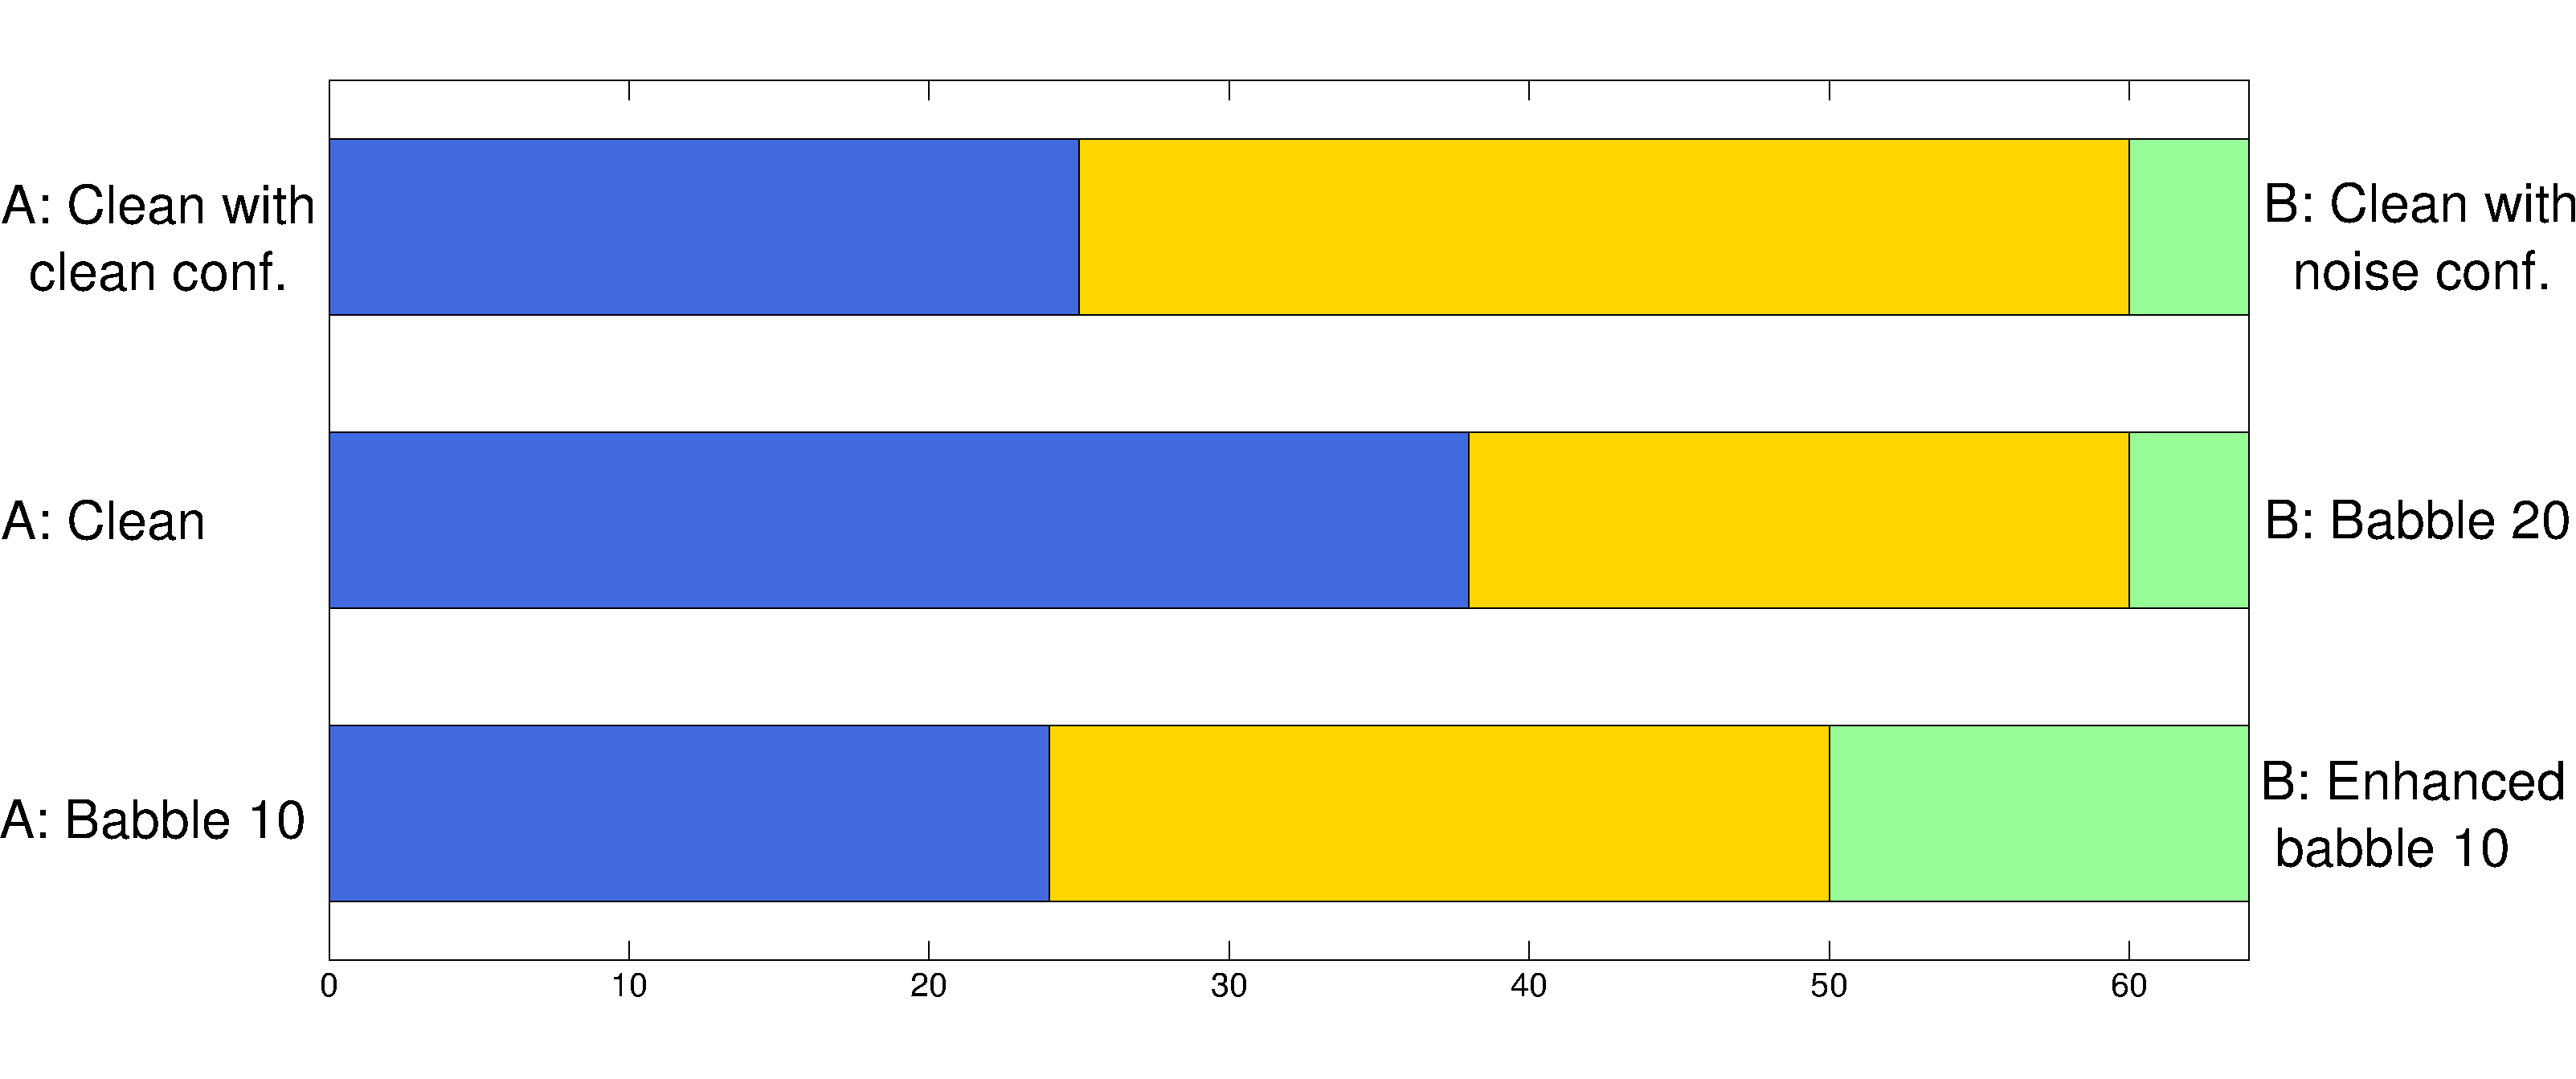
\includegraphics[width=\textwidth]{images/glott_vs_glott.pdf}
  \caption{Results of the AB test comparing different adapted voices obtained with the GlottHMM-based system}
  \label{fig:glott_vs_glott}
  \end{centering}
\end{figure}

In the first two cases, where the adapted voice using clean data and the clean configuration (both samples A) is compared to the one obtained using the noise reduction configuration and babble 20dB data, the results are pretty clear and show a preference to speech using clean data and a clean configuration ($p = 0.043$ and $p \ll 0.0001$).
%
For the third case, no significant conclusion can be formulated.

In Figure \ref{fig:glott_vs_st} the results of the AB test comparing GlottHMM-based system to the STRAIGHT-based are shown.
%
The comparisons made in these tests are all for the cases where babble noise is found on the background, as is the most common noise you could find when recording speech and also one of the hardest ones to deal with, due to its similar nature with speech.

These results show a slight preference for the GlottHMM samples over the STRAIGHT ones in the case of SNR 10dB and 20dB babble noise in the adaptation data.
%
The statistical significance test (binomial test) conducted shows that this preference is only closed to significant at best ( $p = 0.0516$ for SNR 20dB and $p \gg 0.05$ for SNR 10dB).
%
Nothing decisive can be said about the case where the adapted speech was obtained with the enhanced data.

\begin{figure}[!htb]
  \begin{centering}
  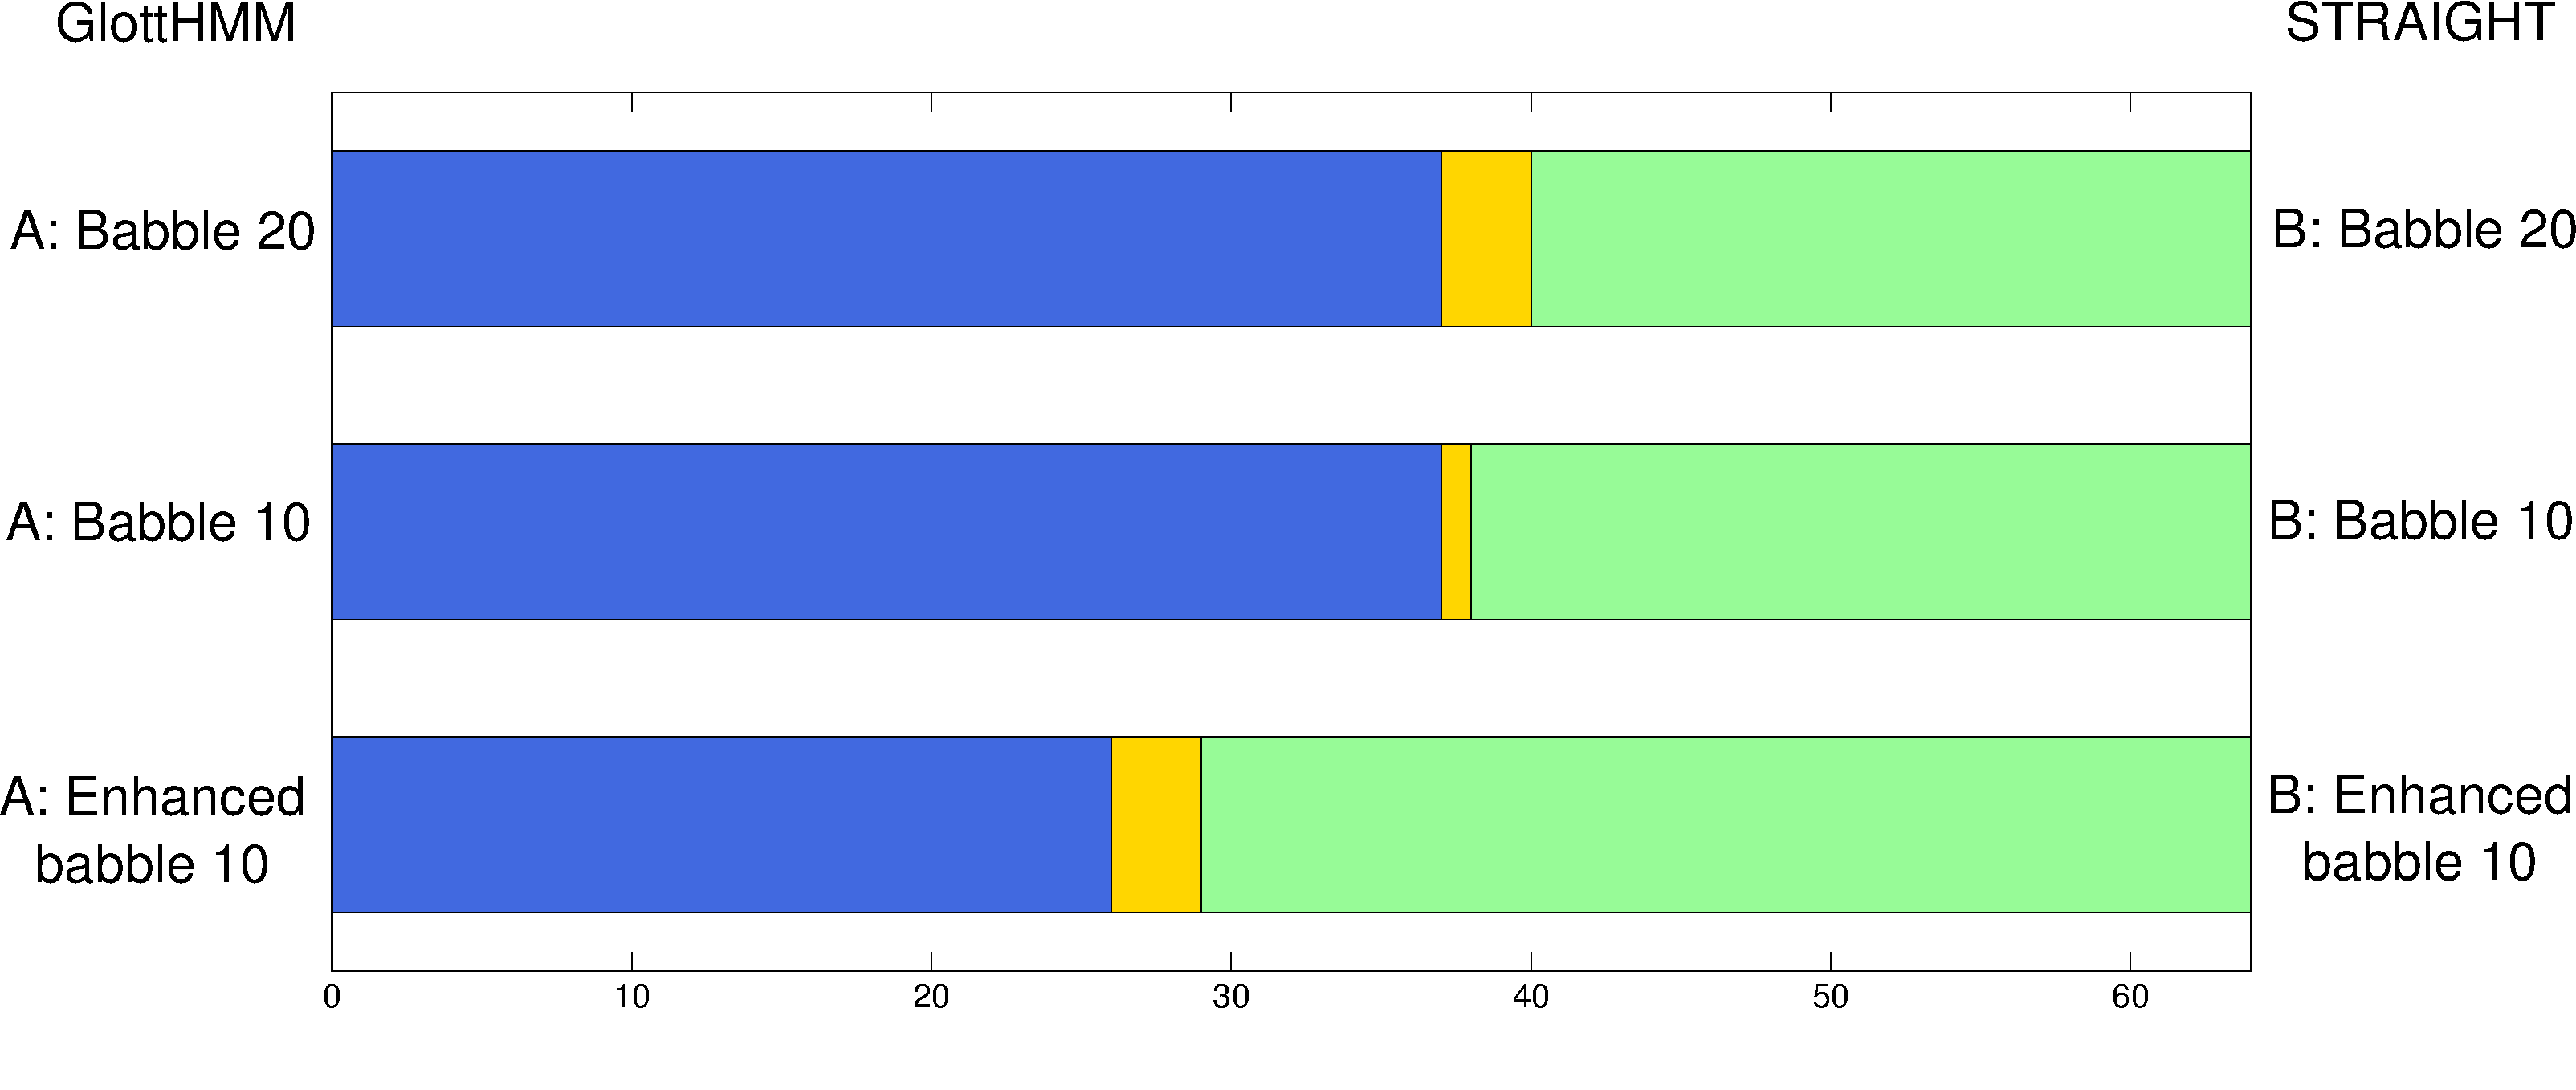
\includegraphics[width=\textwidth]{images/glott_vs_st.pdf}
  \caption{Results for the AB test comparing the performance of the GlottHMM-based system against the STRAIGHT-based one}
  \label{fig:glott_vs_st}
  \end{centering}
\end{figure}

Finally, Figure \ref{fig:mos_scores} presents the MOS scores for the listening test.
%
The STRAIGHT system is rated slightly higher in naturalness than the GlottHMM-based system for almost all the noise cases.
%
In similarity both systems are quite close, with STRAIGHT being slightly better in the case of babble at SNR 20dB.
%
Background quality is rated very evenly for the STRAIGHT-based systems, whereas the GlottHMM is highly affected when the SNR drops from 20dB to 10dB.

\begin{figure}[!htb]
  \begin{centering}
  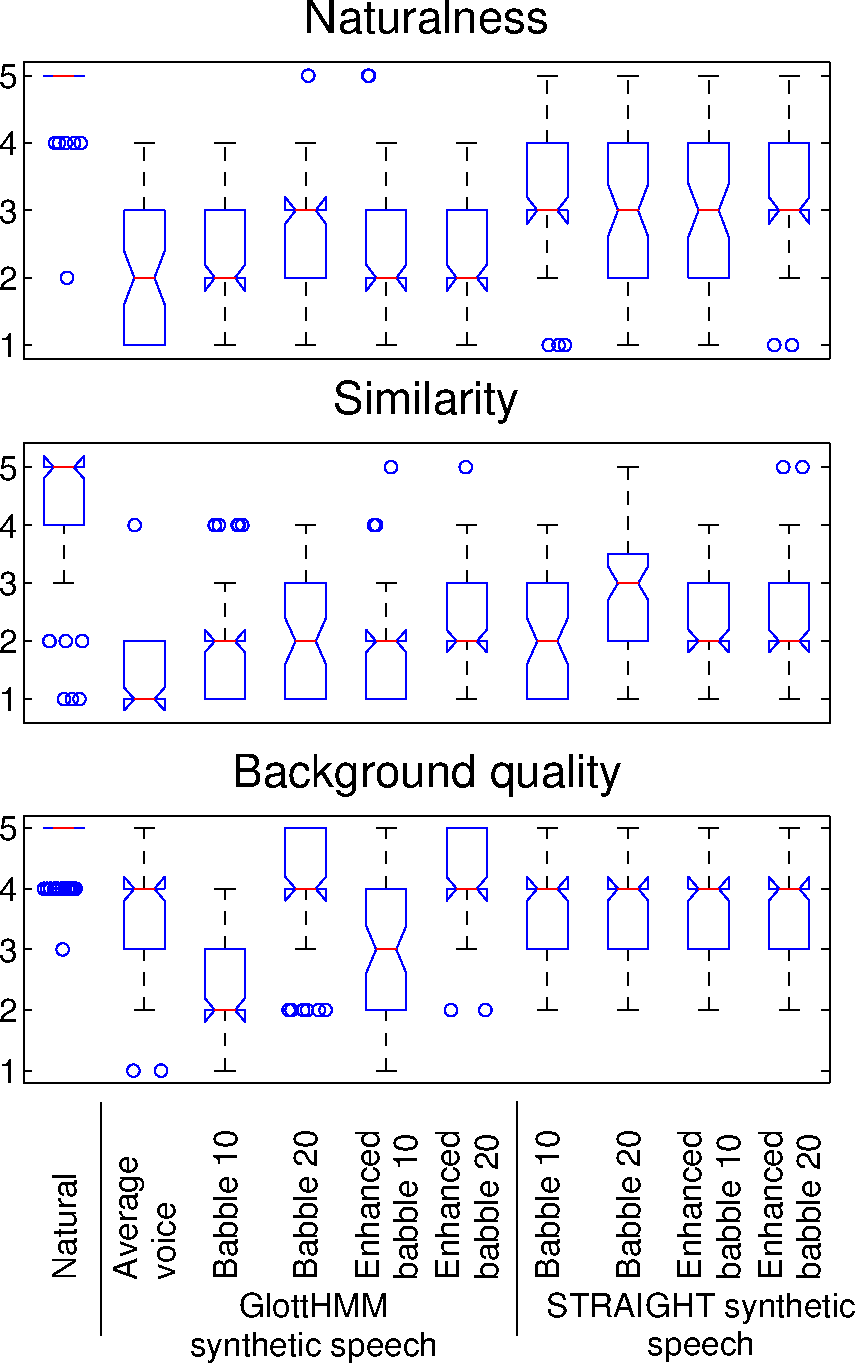
\includegraphics[width=0.75\textwidth]{images/all_subjective_test_quality.pdf}
  \caption{Mean opinion scores (MOS) for the second part of the listening test. Median is denoted by the red line, boxes cover 25th and 75th percent percentiles, whiskers cover the data not considered outliers. The notches mark the 95\% confidence interval for the median}
  \label{fig:mos_scores}
  \end{centering}
\end{figure}